% For copyright and license information, see uiucthesis2021.dtx and derivatives.
\documentclass{uiucthesis2021}
\usepackage[utf8]{inputenc}
\usepackage[inference]{semantic}
\usepackage[english]{babel}
\usepackage{csquotes}
\usepackage{pifont}
\usepackage{stmaryrd}
\usepackage{microtype}
\usepackage{amsmath,amsthm,amssymb}
\usepackage[bookmarksdepth=3,linktoc=all,colorlinks=true,urlcolor=blue,linkcolor=blue,citecolor=blue]{hyperref}
\usepackage[capitalize]{cleveref}
\usepackage[style=ieee]{biblatex}
\usepackage[inline]{enumitem}
\usepackage{dirtytalk}
\usepackage{graphicx}
\usepackage{wrapfig}
\usepackage{subcaption}
\usepackage{listings}
\usepackage{xcolor}
\usepackage{longtable}
\usepackage{tabularx}

% \usepackage{ruledchapters}  % example of compliant heading format, uncomment to use

% uncomment the below to show a grid on all pages
% \usepackage[grid, gridunit=in, gridcolor=blue!40, subgridcolor=blue!20]{eso-pic}

% Settings for listings
\usepackage{algpseudocode}
\newcommand\CONDITION[2]%
  {\begin{tabular}[t]{@{}l@{}l@{}}
     #1&#2
   \end{tabular}%
  }
\algdef{SE}[WHILE]{While}{EndWhile}[1]%
  {\algorithmicwhile\ \CONDITION{#1}{\ \algorithmicdo}}%
  {\algorithmicend\ \algorithmicwhile}
\algdef{SE}[FOR]{For}{EndFor}[1]%
  {\algorithmicfor\ \CONDITION{#1}{\ \algorithmicdo}}%
  {\algorithmicend\ \algorithmicfor}
\algdef{S}[FOR]{ForAll}[1]%
  {\algorithmicforall\ \CONDITION{#1}{\ \algorithmicdo}}
\algdef{SE}[REPEAT]{Repeat}{Until}{\algorithmicrepeat}[1]%
  {\algorithmicuntil\ \CONDITION{#1}{}}
\algdef{SE}[IF]{If}{EndIf}[1]%
  {\algorithmicif\ \CONDITION{#1}{\ \algorithmicthen}}%
  {\algorithmicend\ \algorithmicif}%
\algdef{C}[IF]{IF}{ElsIf}[1]%
  {\algorithmicelse\ \algorithmicif\ \CONDITION{#1}{\ \algorithmicthen}}
\definecolor{codegreen}{rgb}{0,0.6,0}
\definecolor{codegray}{rgb}{0.5,0.5,0.5}
\definecolor{codepurple}{rgb}{0.58,0,0.82}
\lstdefinestyle{mediksty}{
  keywordstyle=\color{magenta},
  commentstyle=\color{codepurple}
}
\lstdefinelanguage{medik}{
  morekeywords={either, or, machine, interface, vars, state, entry, on, do, goto, receives, ~>, =>},
  morecomment=[l]{//},
  morecomment=[s]{/*}{*/}
}

\definecolor{greybackground}{rgb}{0.95,0.95,0.92}
\lstdefinestyle{ksty}{
  keywordstyle=\color{magenta},
  basicstyle=\ttfamily\small,
  commentstyle=\color{codepurple},
  %backgroundcolor=\color{greybackground},
  framerule=0pt
}
\lstdefinelanguage{k}{
  morekeywords={rule,configuration,=>,syntax,multiplicity,type,module,endmodule,import,imports, left,strict,seqstrict,bracket,structural,requires},
  morecomment=[l]{//},
  morecomment=[s]{/*}{*/}
}

\algrenewcommand\alglinenumber[1]{\footnotesize #1} \newcommand{\inlinemedik}[1]{\lstinline[style=mediksty,basicstyle=\ttfamily\footnotesize]{#1}}
\newcommand{\inlinek}[1]{\lstinline[style=ksty,basicstyle=\ttfamily\footnotesize]{#1}}
\lstset{ literate={~}{{\raisebox{0.5ex}{\texttildelow}}}{1} }

\graphicspath{{./figures}}
\addbibresource{./references.bib}

\newcounter{counterforappendices}
\newcommand{\frontend}{\emph{frontend}}
\newcommand{\BPG}{BPG}
\newcommand{\BPGs}{BPGs}
\newcommand{\CGS}{CGS}
\newcommand{\CGSs}{CGSs}
\newcommand{\HCP}{HCP}
\newcommand{\HCPs}{HCPs}
\newcommand{\ED}{ED}
\newcommand{\EDs}{EDs}
\newcommand{\CDSS}{CDSS}
\newcommand{\CDSSs}{CDSSs}
\newcommand{\BPGLogic}{knowledge-base}
\newcommand{\K}{\mathbb{K}}
\newcommand{\MediK}{\text{Medi}\K{}}
\newcommand{\FSM}{\emph{FSM}}
\newcommand{\FSMs}{\emph{FSMs}}
\newcommand{\Var}{\text{Var}}
\newcommand{\LHS}{\emph{\text{LHS}}}
\newcommand{\RHS}{\emph{\text{RHS}}}
\renewcommand{\phi}{\varphi}
\newcommand{\GUI}{GUI}
\newcommand{\UI}{UI}
\newcommand{\UIs}{UIs}
\newcommand{\GUIs}{GUIs}
\newcommand{\PME}{PME}
\newcommand{\PMEs}{PMEs}
\newcommand{\CIG}{CIG}
\newcommand{\CIGs}{CIGs}
\newcommand{\EHRs}{EHRs}
\newcommand{\ACLS}{ACLS}
\newcommand{\CPR}{CPR}
\newcommand{\CISs}{CISs}
\newcommand{\RTSs}{RTSs}
\newcommand{\ASMs}{ASMs}
\newcommand{\DSL}{\text{DSL}}
\newcommand{\DSLs}{\text{DSLs}}
\newcommand{\IT}{IT}
\newcommand{\EHR}{EHR}
\newcommand{\ONC}{ONC}
\newcommand{\NAM}{NAM}
\newcommand{\BNF}{BNF}
\newcommand{\MLM}{\text{MLM}}
\newcommand{\MLMs}{\text{MLMs}}
\newcommand{\GLIF}{\text{GLIF}}
\newcommand{\GEODECM}{\text{GEODE-CM}}
\newcommand{\PCAPE}{\text{P-CAPE}}
\newcommand{\DEGEL}{\text{DeGeL}}
\newcommand{\GLARE}{\text{GLARE}}
\newcommand{\GPROVE}{\text{GPROVE}}
\newcommand{\GOSPEL}{\text{GOSpeL}}
\newcommand{\GEE}{\text{GEE}}
\newcommand{\AAP}{\text{AAP}}
\newcommand{\NHS}{\text{NHS}}
\newcommand{\GP}{\text{GP}}
\newcommand{\GPs}{\text{GPs}}
\newcommand{\SAGE}{\text{SAGE}}
\newcommand{\MPS}{\text{MPS}}
\newcommand{\PC}{\text{PC}}
\newcommand{\PlanSet}{\text{PlanSet}}
\newcommand{\PatientSet}{\text{PatientSet}}
\newcommand{\ConditionSet}{\text{ConditionSet}}
\newcommand{\FinalStateSet}{\text{FinalStateSet}}
\newcommand{\Considered}{\text{Considered}}
\newcommand{\filter}{\text{filter}}
\newcommand{\possible}{\text{possible}}

% Convenience Commands
\newcommand{\cmark}{\text{\ding{51}}}
\newcommand{\xmark}{\text{\ding{55}}}
\newcommand{\greencheck}{{\color{green}\cmark}}
\newcommand{\redcross}{{\color{red}\xmark}}
\newcommand{\cancelcheck}{\bcancel{\cmark}}
\newcommand{\stress}[1]{\underline{\emph{#1}}}

% Scheduling Commands
\newcommand{\Machine}{\mathcal{M}}
\newcommand{\Instance}{\mathcal{I}}
\newcommand{\scheduled}{\textit{scheduled}}
\newcommand{\enabled}{\textit{enabled}}
\newcommand{\epoch}{\textit{epoch}}

% Logic-Related
\newcommand{\antecedent}[1]{\text{antecedent}\left(#1\right)}
\newcommand{\consequent}[1]{\text{consequent}\left(#1\right)}


\begin{document}

\title{A Semantics-First Approach to Clinical Decision Support}
\author{Manasvi Saxena}
\department{Computer Science}
\phdthesis
\degreeyear{2024}
\committee{
  Professor Grigore Ro\c{s}u, Chair \& Director of Research\\
    Professor Lui Sha,
    TBD}
\maketitle

\frontmatter

\begin{abstract}
  Abstract...
\end{abstract}

\begin{dedication}
To my family
\end{dedication}

\begin{acknowledgments}
  Write Here
\end{acknowledgments}

{
    \hypersetup{linkcolor=black}  % disable link coloring locally
    \tableofcontents
    % the Graduate College doesn't recommend including lot or lof
    % \listoftables
    % \listoffigures
}

\chapter{List of Abbreviations}

\begin{abbrevlist}
\item[PCAST]    President's Council of Advisors on Science and Technology
\item[CAST]     Commercial Aviation Safety Team
\item[PME]      Preventable Medical Error
\item[CDSS]     Clinical Decision Support System
\item[BPG]      Best Practice Guideline
\item[HCP]      Healthcare Practitioner
\item[ONC]      Office of the National Coordinator for Health Information Technology
\item[NAM]      National Academy of Medicine
\item[EHR]      Electronic Health Record
\item[BNF]      Backus-Naur Form
\item[MLM]      Medical Logic Module
\item[GEODE-CM] Guided Entry of Data Elements for Clinical Management
\item[GLIF]     Guideline Interchange Format
\item[P-CAPE]   Partners Computerized Algorithm Processor and Editor
\item[DeGeL]    Digital Electronic Guideline Library
\item[GLARE]    Guideline Acquisition, Representation, and Execution
\item[GPROVE]   Guideline PRocess cOnformance VErification Framework
\item[GOSpeL]   Guideline prOcess Specification Language
\item[GEE]      Guideline Execution Engine
\item[AAP]      American Academic of Pediatrics
\item[NHS]      National Health Service
\item[GP]       General Practitioner
\item[SAGE]     Standards-based Guidelines Environment
\item[MBA]      Model-based Architecture
\item[CTL]      Computation Tree Logic
\item[LTL]      Linear Temporal Logic
\item[SOS]      Structural Operational Semantics
\item[AAP]      American Academy of Pediatrics
\item[ITL]      Interval Temporal Logic
\end{abbrevlist}

\chapter{List of Symbols}

\begin{symbollist}[0.7in]
\item[$\tau$] Time taken to drink one cup of coffee.
\item[$\mu$g] Micrograms (of caffeine, generally).
\end{symbollist}

\mainmatter

\section{Introduction}

Preventable Medical Errors (\PMEs{}) characterized by
incorrect intended treatment, or incorrect executions of intended
treatment present a significant challenge in Healthcare
\cite{RodziewiczStatsPearls18}. According to a seminal report on the subject
\cite{DonaldsonBook00}, in 1997,
between 44,000 and 98,000 deaths were estimated to have been caused by \PMEs{} in
the United States alone. A more recent study analyzed data from the eight-year
period between 2000 and 2008, and estimated that in 2013, the number of deaths
caused by \PMEs{} was more than 250,000, making \PMEs{} the third-leading
cause of death in the United States \cite{MakaryBMJ16}.
The adverse effects of \PMEs{} extend beyond patient outcomes.
One study estimated the financial burden of \PMEs{} to the United States to be
19.5 billion dollars in 2008 \cite{AndelJHCF12}. According to the authors of
\cite{RodziewiczStatsPearls18}, \PMEs{} caused psychological effects such
as anger and guilt in healthcare providers (\HCPs{}), adversely impacting their mental
health.

One strategy to mitigate \PMEs{} is to utilize evidence-based statements
published by hospital and medical associations that codify recommended
interventions for various clinical scenarios called Best Practice Guidelines (\BPGs{})
\cite{field1990clinical}. High quality guidelines are routinely updated to account for
 results from clinical trials and advances in medicine, and make the latest
 diagnosis and treatment information accessible to providers \cite{SteinbergNAP11}.

While \BPGs{} have the potential to reduce medical errors, their effectiveness hinges
on the adherence of healthcare providers to them.
For example, consider Advanced Cardiac Life Support (\ACLS{}): a \BPG{} published
by the American Heart Association (AHA) for management
of a life threatening condition called in-hospital cardiac arrest (IHCA) \cite{AHAGuidelineAdult, AHAGuidelinePed}. Studies suggest that management
of IHCA in 30\% of adult, and 17\% of pediatric cases deviates from the
AHA-prescribed \BPG, resulting in worse patient outcomes \cite{Ornato2012DeviationAdult,Wolfe2020DeviationPediatric,
Crowley2020DeviationAdult,Honarmand2018Adherence,Mcevoy2014Adherence}.

\begin{wrapfigure}{l}{0.5\textwidth}
  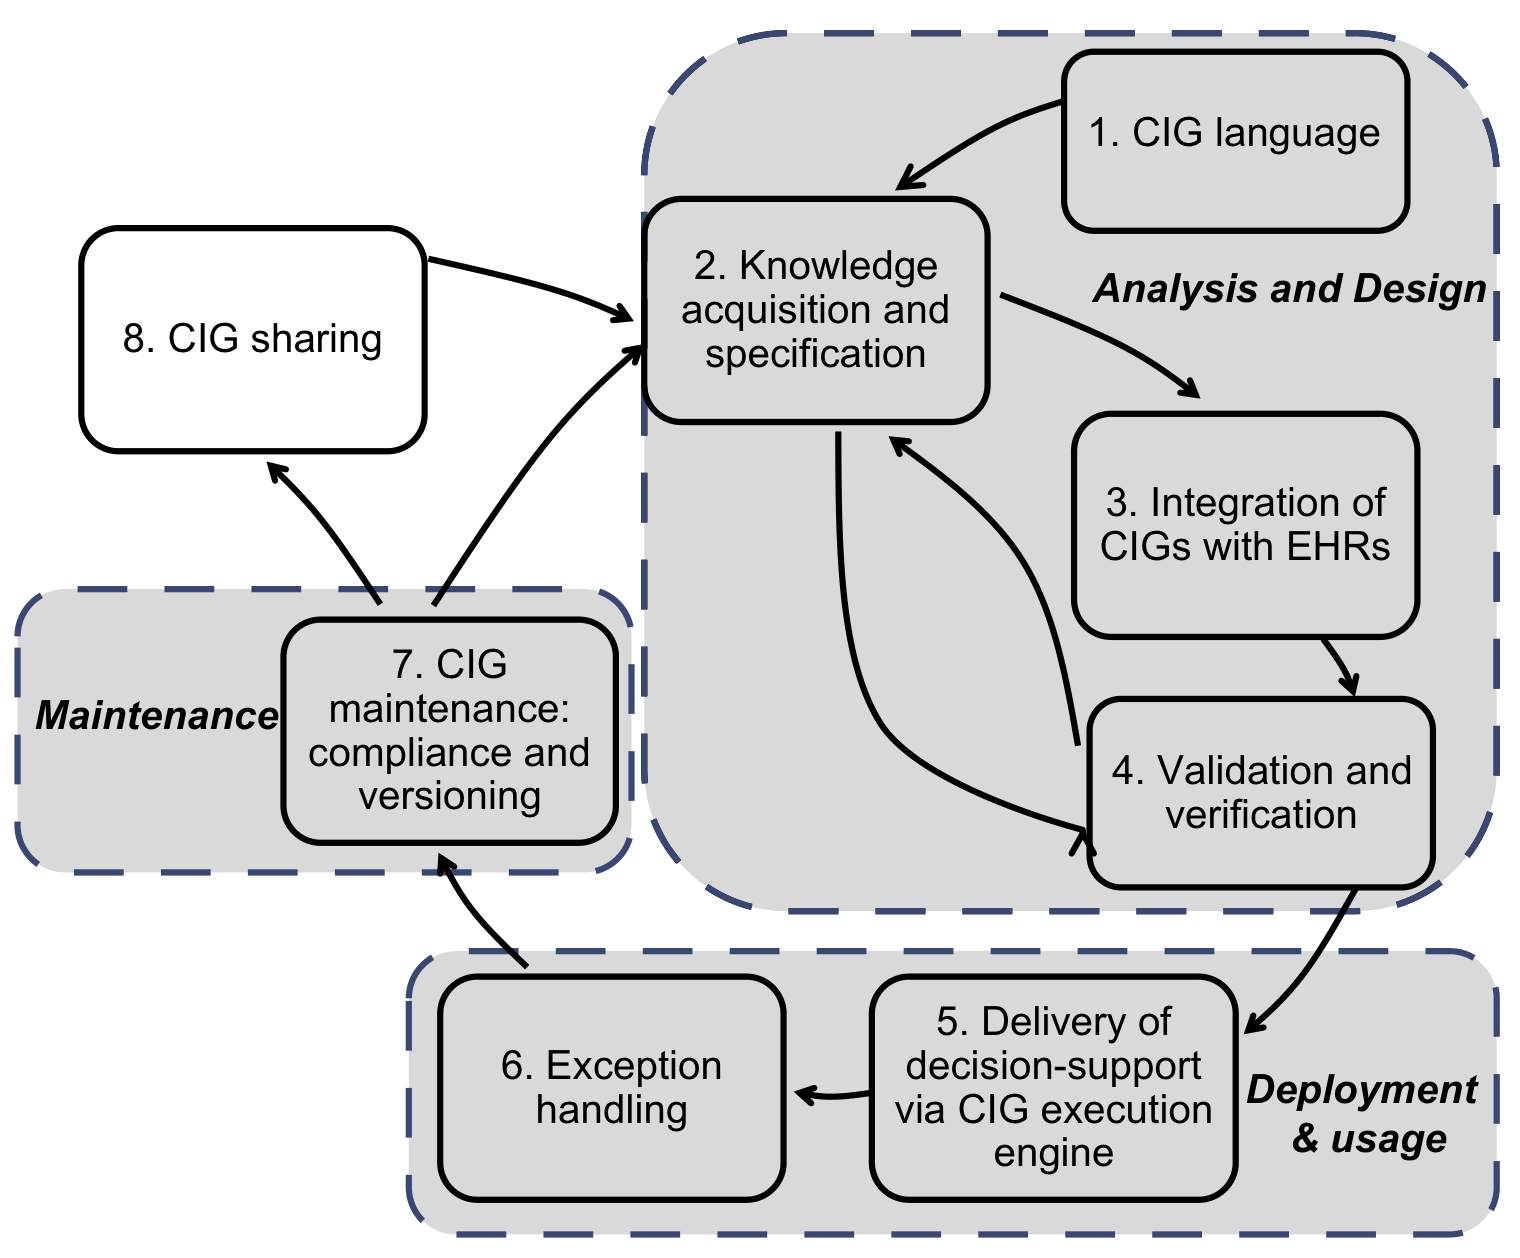
\includegraphics[width=\textwidth]{cpg-topics}
  \caption{\CDSSs{} Research Themes}\label{fig:cpg-research-topics}
\end{wrapfigure}

While \BPG{}-adherence is difficult to achieve in
practice \cite{RandJAMA99,DavisCMAJ97},
integrating \BPGs{} with existing patient care-flow,
and making them readily-accessible when required can improve adherence \cite{WoolfBMJ99}.
To this end, hospitals commission computerized Decision Support Systems (\CDSSs{})
that codify \BPGs{} and support \HCPs{} with situation-specific advice.
Such systems have been shown to improve \BPG{}-adherence \cite{GargJAMA06,KawamotoBMJ05}, and evidence from multi-center clinical trials
suggests that they reduce \PMEs{} \cite{BenettJAMIA16,SahotaJIS11}.
Thus, guideline-based \CDSSs{} are now considered imperative to the
future of medical decision making in general \cite{JamesNEJM01}.

While the potential of \CDSS{} has been recognized, wider adoption
is still hampered by significant challenges. \CDSSs{} are safety-critical -
bugs can have serious (sometimes life-threatening) consequences.
Thus, it's vital that:
\begin{enumerate*}[label=(\alph*)]
  \item the system is formally verified to satisfy desired correctness
    properties, and,
  \item \HCPs{} can trust the medical knowledge embedded in the system.
\end{enumerate*}
While research on \CDSSs{} has resulted in progress towards addressing
these challenges, more work is needed to realize their full potential.
We briefly provide an overview of existing research on \CDSSs{} to explain
both progress made and challenges remaining in context of \CDSSs{}.
In \cite{PelegJBI13}, the author provides a methodological review of
existing work on Computer Interpretable Guidelines (\CIGs{}): executable
formalizations of \BPGs{} used to construct \CDSSs{}.
Existing work is classified into one of eight themes spanning
the entire development cycle of a \CIG{}. The themes and relations between them
are shown in \figurename{} \ref{fig:cpg-research-topics}.

According to the author in \cite{PelegJBI13}, \CIGs{} are usually based on previously published non-executable
\BPGs{}. To develop a \CIG{}, a language is identified in (1). Teams of
software developers and clinicians then collaborate to express medical knowledge
in the \BPG{} in the identified language. In (3), the \CIG{}
is integrated with components such as a Graphical User
Interface (\GUI{}), Electronic Health Records (\EHRs{}) and external devices
(such as monitors for patient parameters) to obtain a \CDSS. Before adoption
in the real-world, it is imperative to ensure that the \CIG{} \emph{mirrors}
the underlying \BPG{}. This validation occurs by \emph{testing} the \CDSS{}
using execution capabilities of the modeling language from (1) in (5).
Additionally, formal verification may be used to establish other desired
properties hold. Inconsistencies identified in (5) are fixed through developer-clinician
collaboration in (2),  re-validation and
verification. While the aforementioned development cycle has resulted in several
effective \CDSSs{}, it has some limitations:

\paragraph{Gap between specification and implementation:}

To develop the \CIG{}, software developers rely on clinicians to interpret the
non-executable \BPG{} and communicate
the intended semantics to them. Thus, the non-executable \BPG{} serves as a functional specification for
the \CIG{}, i.e. the implementation. In such safety-critical systems, it is
imperative that the implementation, i.e. the \CIG{}, conforms to its
specification, i.e., the \BPG{}. To address this, the \CIG{} is tested by
putting the \CDSS{} through clinical simulations. But, while testing reduces
the risk of non-conformance, it does not completely eliminate it.

%\paragraph{Safe Modularity:}
%
%While developing \CDSSs{} is both complex and cost-intensive,
%the development effort can be reduced by sharing \CDSSs{} across hospitals \cite{PelegAMIA00}.
%But, even for the same \BPG{}, hospitals develop their own \CDSSs{} to address
%their needs, resulting in duplicated work.
%For instance, for the \ACLS{} \BPG{}, multiple \CDSSs{} have been developed by different
%different hospitals in a span of just six years years \cite{FullCodePro,PediAppRREST2020,
%PediAppRREST2021,GuidingPad2017,GuidingPad2019, GuidingPad2020,DST2014,DST2019,ROSCo2021,TeamScreen2019,Wu2017}.
%\CDSSs{} based on the same \BPG{} typically have the same \CIG{}, but may differ
%in their Graphical User Interfaces (\GUIs), or integration with external
%devices, to address hospital-specific needs.
%To enable safe sharing of knowledge, we need a mechanism that:
%\begin{enumerate*}[label=(\alph*)]
%  \item allows a stable, formally-verfied \CIG{} that is \emph{decoupled} from other
%    components, and,
%  \item supports hospital-specific customizations without compromising system
%    \emph{safety}.
%\end{enumerate*}


\paragraph{Formal semantics and analysis tools:}

Given the safety-critical nature of \CDSSs{}, it is vital for \CIG{} languages
to have complete formal semantics and formally-verified execution engines and
analysis tools. This need has already been recognized in existing literature
\cite{SuttonAMIA03, ShaharAMIA96}. It's also vital to ensure that
associated tools are kept up to date as the language evolves.

\paragraph{Holistic system safety:}

While the safety critical nature of \CDSSs{} neccessitates
\CIG{} languages to have comprehensive support for verification using
tools like model checkers and deductive verifiers, certain challenges
specific to \CDSSs{} require support beyond traditional techniques.

Actions performed by a \CDSS{} can either be \emph{programming-oriented}
or \emph{clinically-oriented} \cite{BoxwalaJBI04}. \emph{Programming-oriented}
actions are peformed by executing the \CIG{} itself. For example,
using patient parameters, or health records to make a reccomendation or diagnosis,
or to raise a warning. \emph{Clinically-oriented} actions on the other hand
are ones that involve a clinician. For example, in the case of \ACLS{},
the \CDSS{} recommends that Cardiopulmonary Resuscitation (\CPR{}) be performed
for a certain length of time. Such actions can only be performed by clinicians,
an the \CDSS{} assumes that the recommended action was indeed performed before
moving resuming guidance.

For correctness, both categories of actions must be completed
successfully. While traditional formal reasoning techniques can be employed
to establish correctness of \emph{programming-oriented} actions, the same
cannot be used to reason about \emph{clinically-oriented} ones.
Thus, a mechanism that allows some guarantees about clinically-oriented is
desirable.

This proposal aims to address these limitations comprehensively
using a \emph{semantics-first} approach.
By \emph{semantics-first}, we mean that \CIG{} language we
use to is formally defined, from which tools such as an interpreter, model checker,
and deductive verifier are derived in a \emph{correct-by-construction}
manner. At the core of our approach is new language Domain Specific Language (DSL)
for \CIGs{} called \MediK{}. By emphasizing \HCP{}-\emph{comprehensibility},
\MediK{} enables \HCPs{} to verify the semantic correctness of a \CIG{}.
\MediK{} provides a uniform way of modeling diverse external agents, enabling reasoning about
safety of the entire system.

\MediK{} has been used to implement a real-word \CDSS{} for screening and
mangement of pediatric sepsis, and establish said \CDSS{} satisfies desired
safety properties. To the best of our knowledge, it is the first system
for sepsis management with formal safety guarantees.

While \MediK{} presents a promising direction towards developing safe real-world
systems, realizing its full potential requires addressing the following research
challenges (RCs):

\paragraph{RC 1 (Design):} Is \MediK{}'s design conducive to expressing diverse \BPGs{}?

\BPGs{} can vary greatly by scope and purpose. For instance,
consider differences between the \BPGs{} for managing cardiac
arrest and sepsis. The \BPG{} for cardiac arrest can be
succinctly depicted by a single workflow. On the other hand, the \BPG{} for
screening and management of sepsis involves multiple workflows with complex
inter-workflow interactions.
This proposal seeks to answer whether \MediK{}'s
design can adequately accomodate diversity in \BPGs{}, without
compromising on readability. To this end, we plan to collaborate with
experts in medicine to ensure that the language meets their needs.
Note that the \emph{semantics-first} approach is particularly
well-suited for designing the language, as updates to the language
only require changes to the semantics. As tools are derived from the semantics,
they update automatically.

\paragraph{RC 2 (Ecosystem):} Does \MediK{} have a mature
set of tools that enable building safe \CDSSs{}?

\MediK{} has a complete executable formal semantics, from which
its tools are derived in a \emph{correct-by-construction} fashion.
But, as real-world \BPGs{} are complex, establishing appropriate safety and liveness properties using
said tools presents various challenges. The proposal seeks to build on
\MediK{}'s toolchain to support verification of desired safety and liveness
properties of large \BPGs{}.

While $\K$ derived tools enable execution and analysis of \MediK{} programs,
certain \BPG{}-specific requirements may not have direct $\K{}$ equivalents.
In such cases, this proposal seeks to develop new semantics-based tools within
the $\K{}$ ecosystem, that are vital in \MediK's context, but may also have
applications for other $\K$-based languages.
For instance, visual representations of \MediK{} programs can
significantly improve comprehensibility of \MediK{} programs to medical domain
experts. This proposal seeks to expand on techniques
such as semantics-based compilation that can be used to extract information such
as basic blocks from code to generate \emph{correct-by-construction} visual
representation of programs in any language.

\paragraph{RC 3 (Applications):} Can \MediK{} be used to build real-world
\CDSS{}? How can \MediK{} improve \CDSSs{} effectiveness?

This proposal
seeks to establish that our approach can be used to build systems with real
world applications. To this end, we plan to build \CDSSs{} that are
capable of consideration for clinical trials at hospitals. Note that we
intend to use clinical-trial worthiness as an indicator of the effectivenss
of \MediK{}, not the result of the trial itself.
Clinical-trial worth systems need to be integrated into existing hospital care-flow.
This involves handle hospital-specific variations, such as
diversity in data sources and health records. This proposal seeks to
develop the \MediK{} ecosystem to a point where it can be used to build
such systems.

This proposal also seeks to develop new \CDSS{} capabilities enabled by the
\emph{semantics-first} approach. In particular, our approach
enables the following capabilities:

\begin{itemize}
  \item \textbf{Guideline Adherence Proofs:} Execution of a
\MediK{} \BPG{} is simply a proof in Matching Logic (ML), the logic
underlying the $\K{}$ framework, using the semantic rules as axioms.
Said proofs can be checked by an external ML proof-checker.
In \MediK{}'s case, execution proofs can serve as evidence of adherence to best practices during treatment.
Moreoever, zero-knowledge proofs can allow hospitals to establish
conformance to best practices, without divulging sensitive information
such as \emph{patient data} or \emph{specific treatment}
  \item \textbf{Safe Incorporation of Artificial Intelligence (AI):}
Advances in AI have applications in medicine. AI-based components
can enable early detection and targed treatment of medical conditions.
However, integrating such systems \emph{safely} remains a challenge,
\emph{hallucinations} in AI-based systems can lead to serious consequences.
We seek to explore \emph{safe} incorporation of AI-based systems into cafe-flow using
a simplex-based approach, where recommendations from an AI-based component are
\emph{checked} against known best practices before they're enacted.
If the recommendation is determined to be unsafe, a fallback action is enacted
instead.
\end{itemize}



\chapter{Background}

This chapter introduces relevant background information on
best practice guidelines (\BPG{}) and guidelines-based clinical decision support
systems (\CDSS{}).
In section \ref{sec:bpg-background}, we utilize a real-world \BPG{}
to explain the motivation behind codifying treatment
in the form of clinical guidelines. We also briefly discuss
common characteristics of such guidelines that enable medical knowledge
to be represented efficiently and accurately.

\BPGs{} are usually published by hospitals,
research institutions and medical associations with the aim to improve quality of care by
\begin{enumerate*}[label=(\alph*)]
  \item reducing medical errors due to preventable causes,
  \item standardizing knowledge from latest evidence-based research, and,
  \item enabling access to aforementioned knowledge at medical establishments
  that lack resources to conduct research.
\end{enumerate*}

While in theory, following \BPGs{} should improve clinical outcomes,
their effectiveness in practice is dictated by whether healthcare practitioners
follow them or not. In section \ref{sec:cdss-background}, we present
challenges that practitioners encounter in following \BPGs{}. We then argue
that non-conformance results in worse patient outcomes.
Next, we show how computerized systems that utilize data from available
heterogeneous sources such as electronic health records and sensors for
patient parameters can improve patient outcomes by addressing challenges
to following \BPGs{} encountered by practitioners.

\section{Clinical Best Practice Guidelines}\label{sec:bpg-background}

Clinical best practice guidelines are evidence-based statements
published by hospital and medical associations that codify recommended
interventions for various clinical scenarios
\cite{field1990clinical}. High quality guidelines are routinely updated to account for
 results from clinical trials and advances in medicine, and make the latest
 diagnosis and treatment information accessible to providers \cite{SteinbergNAP11}.

\begin{figure}[b!]
  \centering
  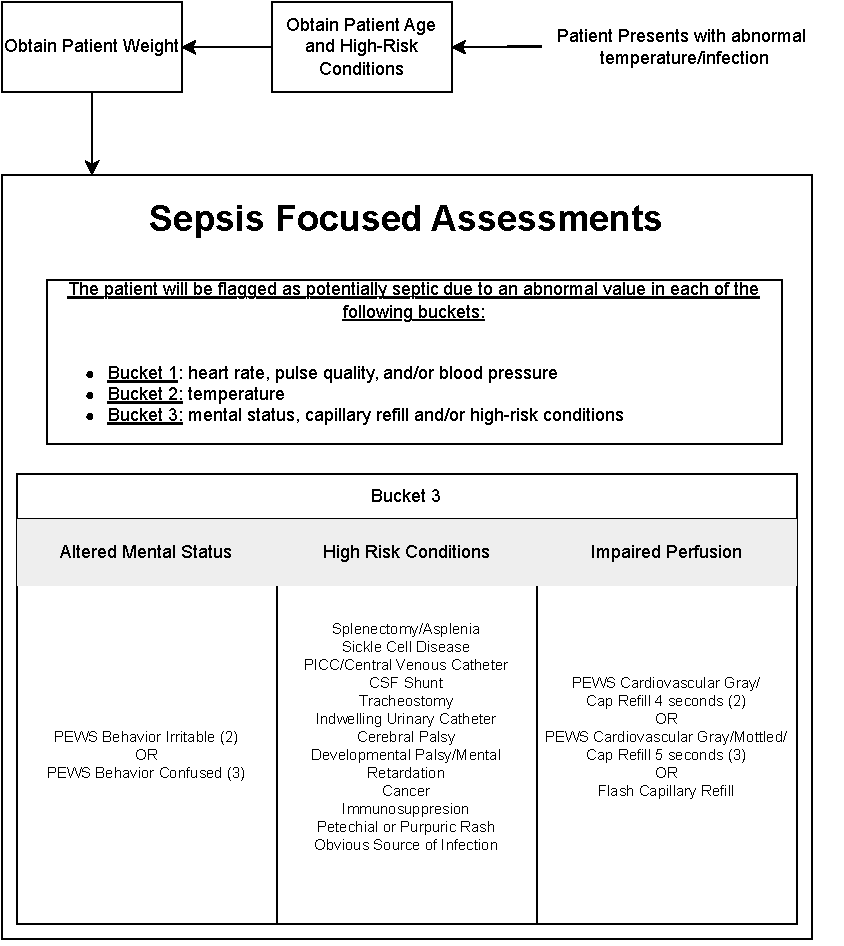
\includegraphics[width=0.43\textwidth]{sepsis-screening-osf}
  %\includegraphics[width=0.5\textwidth]{screening-vitals}
  \caption{Pediatric sepsis screening \BPG{}}\label{fig:sepsis-screening}
\end{figure}

To illustrate characteristics of \BPGs{}, we briefly go over a \BPG{}
for managing sepsis in pediatric cases used at OSF St. Francis Medical Center
in Peoria, Illinois -- a major pediatric hospital in the United States. Note
that for brevity, we refer to said hospital simply as OSF in the remainder of
this section.
Sepsis is life-threatening condition caused by the body's extreme response to
an infection \cite{RhodesICM17}, and is
a major cause of morbidity and mortality in children \cite{Eisenberg2021JP}.
Adverse outcomes can, however, be mitigated through timely
identification and prompt treatment with antibiotics and
intravenous (IV) fluids \cite{Weiss2014CCM,Evans2018JAMA}.
\BPGs{} for screening and management of sepsis in pediatric Emergency
Departments (EDs) have shown effectiveness in screening and management of sepsis \cite{Eisenberg2021JP},
leading to their adoption in many pediatric EDs \cite{Balamuth2017EM,Sepanski2014FP}.

In \figurename{} \ref{fig:sepsis-screening}, we present a simplified version of
the screening section of OSF's sepsis mangement guideline.
In essence, when a patient arrives at the
\ED{} with a fever or an infection, the \HCP{} is supposed to obtain
\begin{enumerate*}[label=(\alph*)]
  \item the patient's age,
  \item any conditions, such as cancer, immunosuppresssion, etc,
    that increase likelihood of sepsis, and
  \item the patient's vital signs, such as heart rate, systolic blood
    pressure, respiratory rate, etc.
\end{enumerate*}
\begin{footnotesize}
  \begin{table}
    \centering
    \begin{tabular}{ | c || c | c | c | }
      \hline
      \textbf{Age}            & \textbf{Heart Rate}   & \textbf{Systolic BP} & \textbf{Temp}  \\
      \hline
      $0d - 1m$               & $>205$                & $<60$                & $<36 \text{ or } >38$ \\
      \hline
      $\geq 1m - 3m$          & $>205$                & $<70$                & $<36 \text{ or } >38$ \\
      \hline
      $\geq 3m - 1y$          & $>190$                & $<70$                & $<36 \text{ or } >38.5$ \\
      \hline
      $\dots$                 & $\dots$               & $\dots$              & $\dots$ \\
      \hline
      $\geq 13y$              & $>100$                & $<90$                & $<36 \text{ or } >38.5$ \\
      \hline
    \end{tabular}
    \caption{Vital Signs Chart}\label{table:vital-signs}
  \end{table}
\end{footnotesize}

This information is then used to check for abnormalities
in clusters of linked information, called \say{buckets}. For instance, if
the patient's heart rate is abnormal, then \say{bucket 1} is said to
have an abnormal value.
Checking for such abnormalities often involves the use of tables, such as
\tablename{} \ref{table:vital-signs} that contains normal ranges indexed by
\emph{age}.
%\footnote{For brevity, we omit some age ranges and vital signs from table
%\ref{table:vital-signs}}.
If the patient has at least one abnormal value in every \say{bucket},
then he/she is flagged as potentially septic.

The \BPG{}-recommended treatment for
sepsis involves multiple concurrent workflows, such as
screening for septic shock, fluid resuscitation, and administering antibiotics.
In \figurename{} \ref{fig:fluid-therapy}, we provide
a version of the fluid resuscitation guideline used
at OSF. Briefly, if the patient is flagged as potentially septic, the guideline suggests
\begin{enumerate*}[label=(\roman*)]
  \item obtaining any fluid-overload risks,
  \item administering normal saline (typically over a period of 15 minutes),
    where the dosage is dictated by risks determined in previous step,
  \item assessing signs of fluid-overload,
  \item evaluating patient responsiveness to normal saline upon completion of
    the administering process, and,
  \item determining whether another fluid bolus should be administered based on
    information from previous steps.
\end{enumerate*}
\begin{figure}[b]
  \centering
  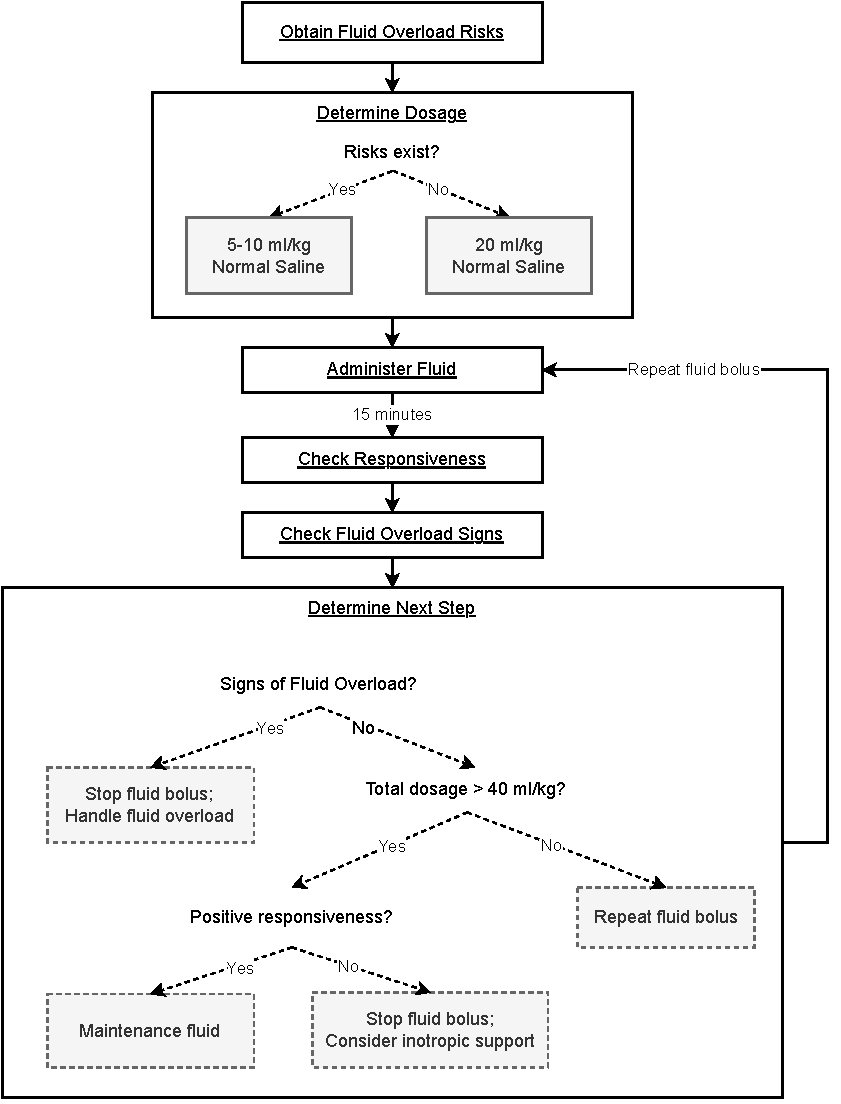
\includegraphics[scale=0.45]{FluidWorkflow-fmcad.pdf}
  \caption{Fluid Resuscitation Guideline}\label{fig:fluid-therapy}
\end{figure}

This real-world \BPG{} exhibits characteristics common
across many \BPGs{}. Specifically \BPGs{} typically:
\begin{itemize}
  \item Involve \stress{concurrent} workflows, such as administering drugs,
    monitoring vitals, performing treatment, etc. There may also be
    inter-workflow interactions. For instance, a diagnosis of sepsis during the
    screening may require modifications to an ongoing course antibitiotics.
  \item Often specified in a \stress{flowchart-like}
    notation. See \cite{AHAFlowcharts} and \cite{CancerCareFlowcharts} for other flowchart-based \BPGs{} for management of \emph{cardiac arrest}, and
    screening, risk-reduction, treatment and survivorship in
    cancer care respectively.
  \item Require communication between \stress{heterogeneous agents} such as
     monitors and Electronic Health Records (EHRs).
  \item Often use \stress{tables} indexed by parameters such as age, weight,
    etc to present normal/abnormal ranges for measurements, or recommended dosages for drugs.
\end{itemize}

Note that the aforementioned characteristics are \emph{not} specific
to one guideline. According to a review paper on \CIGs{} \cite{ClerqAIM03},
such \DSLs{} should additionally
\begin{enumerate*}[label=(\alph*)]
  \item be formally defined, i.e, have a formal syntax and semantics, and
  \item have an execution engine to provide decision support.
\end{enumerate*}


\section{Clinical Decision Support Systems}\label{sec:cdss-background}






\chapter{Hurdles to \CDSS{} Adoption}\label{chapter:hurdles-cdss-adoption}

There is now increasing evidence to suggest that
well implemented \CDSSs{} can significantly improve quality of care
\cite{GargJAMA05,WellsEJPC08}. However, despite several advantages,
several challenges continue to inhibit wider \CDSS{} adoption \cite{Nam17}.
Some challenges are non-technical, i.e., require changes to legislation,
incentive mechanisms and practitioner education and training, and are beyond the
scope of this work. But, several limitations in existing \CDSS{} technology have also
inhibited further adoption. This chapter discusses said challenges, and
the progress made by existing state of art towards addressing them.

Recall, from section \ref{sec:hurdles-cdss-adoption}, that in 2017,
the National Academy of Medicine published a report on \CDSSs{} that
laid out a roadmap to optmize \CDSS{} uptake in medicine. According to the
report, several challenges need to be tackled for wider adoption, such as:


\begin{enumerate}[label=C\arabic*.]
\itemsep0.0em
\item Absence of systematic ways of \emph{validating content}
in a \emph{reliable}, \emph{accessible} and \emph{updateable} manner.
\item Lack of \emph{reliable}, \emph{shareable} \CDSS{} content
that can be easily adopted across healthcare organizations and their (Information
Technology) \IT{} systems.
\item Technical difficulties of sharing due to \emph{need for
  adaptation} to diverse Electronic Health Records (\EHR) systems.
\item \emph{Suboptimal} User Interfaces (\UIs), implementation choices and
workflows.
\end{enumerate}

\section{Addressing Adoption Hurdles}

\CDSS{} first appeared in the 1960s, and have evolved over time
to address aforementioned challenges. The following sections
describe progress made towards addressing aforementioned challnges.

\subsection{Monolithic \CDSSs{}}\label{sec:monolithic-cdss}

Early \CDSSs{} were developed as monolithic standalone systems
that were self-contained, requiring direct user input for clinical data
\cite{RodriguezBook16}. Such systems co-existed with
primitive electronic health records (\EHR{}) systems,
and thus had to rely on manual data entry before administering support.

Several successful \CDSSs{} implementations utilized a standalone
architecture. Early \CDSS{} implementations
such as MYCIN \cite{ShortliffeBook12} required the \HCP{}
to answer a set of questions to provide advice regarding microbial therapy.
Other early \CDSSs{} such as DXplain \cite{BarnettJAMA87} utilized a wide
range of findings (history, data, etc.) to come up with a diagnosis, and
is still in active development.

The reliance on manual entry made using such systems time-consuming. As support for \EHR{} matured,
\CDSSs{} implementations became better integrated with \EHR{} systems
for automated clinical data retrieval.
However, with monolithic systems, the integration was usually \EHR{}-specific \cite{RodriguezBook16}.
Migrating or sharing \CDSS{} content across medical establishments
presented significant challenges as a system designed
for an establishment's \EHR{} system couldn't be used with a different
establishment's \EHR{} system \cite{KawamotoJBI10}.

\subsection{Modular \CDSS{} Architectures}\label{sec:modular-architectures}

In section \ref{sec:cdss-components}, we presented the components that
every guidelines-based clinical decision support can conceptually be decomposed
into. Early \CDSSs{} from section \ref{sec:monolithic-cdss}
were not designed with modularity that enabled sharing components
between different implementations. As the need for scaling \CDSSs{}
across institutions grew, component-based architectures that
enabled \EHR{} agnostic systems to be developed became prevalent \cite{KawamotoJBI10}.

\EHR{}-agnostic architectures represent a significant step towards
addressing several challenges. Such architectures
address C3 as the knowledge-base can be shared across institutions with
different \EHR{} systems. C2 is partially addressed as the
knowledge-base can be independently developed, maintained and distributed.
C4 is also partially addressed as decoupled components, such as the \UI{},
are easier to adapt to \HCP{} preferences.

Over the years, several \CDSS{} implementations have utilized a
components-based architecture. For instance, in \cite{KawamotoJBI10}, the
authors utilize the service-oriented architecture \cite{ErlBook05} to build
a \CDSS{} web service that can be utilized in a completely \EHR{}-agnostic way.
Recent efforts include \CDSSs{} platforms such as
EvidencePoint that enable \CDSS{} to be integrated
closely with the hospital's \EHR{} without being tightly coupled \cite{SolomonJMIR23}.
\EHR{}-agnostic architectures allow decision support to be administered using the
\EHR{}'s \UI{}. Given their prevalence in modern medical establishments,
\EHR{} systems have become integrated into workflows,
and HCPs are accustomed to using them. Dispensing clinical decision
support through the \EHR{}'s \UI{} is vital for adoption, as better workflow
integration can lead to higher adoption \cite{PressJMIR16,LiJMI16}.

Approaches that utilize a component-based architecture
enable medical knowledge to be shared more efficiently.
But, it's possible for medical knowledge itself to be incorrectly
encoded. \BPGs{} are generally expressed as long textual documents meant to
be understood by \HCPs{} \cite{SchiffmanYMI13}. To build a \CDSS{}, the \BPG{} has to be
systematically expressed in a computable medium. This translation process,
referred to as knowledge formalization, is generally ad-hoc, and can be
the source of inconsistencies in encoded medical knowledge
resulting in \CDSSs{} that render wrong advice \cite{ShaharIOS04}.

Typically, in order to translate textual guidelines to a computable
medium, experts in medicine collaborate with computer scientists and
software developers to come up with a requirements document.
This is subsequently utilized to develop the knowledge base, i.e.,
the computer interpretable encoding of the \BPG{} \cite{PelegJBI13} in a
traditional programming language. Thus, the \BPG{} as a
functional specification for the knowledge base.
For instance, in the case of the aforementioned EvidencePoint,
the knowledge base is expressed in  Javascript \cite{SolomonJMIR23}.

However, since computer scientists/software
developers don't understand medicine, and experts in medicine typically
don't understand programming languages,
it's possible for the functional specification, i.e., the \BPG{}, to
diverge from its implementation, i.e., the knowledge base. Thus,
C1 from section \ref{chapter:hurdles-cdss-adoption} remains unaddressed.

\subsection{Computer-Interpretable \BPGs{}}\label{sec:computer-interpetable-bpg}

\CDSSs{} are safety-critical systems, where bugs can have serious consequences.
Thus, ensuring correctness of \CDSSs{} is vital to widespread adoption.
To ensure bugs arising out of divergences between the textual \BPG{}
and its computable translation, i.e., the knowledge base, the gap between
the \BPG{} and the knowledge base must be eliminated. To this end, instead of
encoding \BPGs{} in a conventional programming language, domain-specific
languages (\DSLs{}) for directly expressing \BPGs{} in a computer-interpretable manner can
be utilized. By emphasizing comprehensibility to \HCPs{}, these \DSLs{} enable
\HCPs{} to validate the accuracy of encoded medical knowledge.
A computer-interpretable \BPGs{} can both as the specification, i.e. the textual \BPG{},
and the implementation, i.e., the knowledge base, thereby eliminating the
specification-implementation gap.

In 1989, the Arden Syntax was developed as a result of incompatibility
of medical knowledge between medical institutions \cite{HripcsakCBM94}.
While it was designed to represent simple guidelines,
such as those related to reminders, more complex treatment protocols couldn't
be represented. Arden syntax had a formal Backus-Naur Form (\BNF{})
syntax definition, but no formal semantics, or a standardized execution engine.
Instead, ad-hoc execution engines for the language have been developed over
time \cite{ClerqAIM03}.

Shortcomings regarding ability of the Arden Syntax to represent complex
treatment protocols were addressed by formalisms such as GLIF \cite{PelegAMIA00}
that permit encoding complex guidelines through the use of a multi-layer
approach to represent both high-level medical knowledge and low-level
implementation details. However, just like the Arden Syntax, GLIF lacks
a formal semantics or formal analysis tools.

The need for formal analysis is identified by Asbru: a formalism with formally
defined syntax and semantics \cite{ShaharAMIA96}. In Asbru, a guideline is modeled as a plan
that contains:
\begin{enumerate*}[label=(\roman*)]
  \item intentions that define aims,
  \item conditions that specify when the plan is applicable,
  \item effects that define expected behavior during execution, and,
  \item a body containing other subplans.
\end{enumerate*}
Apart from an execution engine, the Asbru ecosystem also contains
other tools, such as a model checker for verification \cite{BaumlerSPIN06}.
However, the formal semantics of Asbru have been only partially defined, and
is insufficient to implement tools for the language \cite{SuttonAMIA03}.
The importance of a complete formal-semantics is identified and addressed
by PROforma \cite{SuttonAMIA03}, another formalism that uses plans to
model guidelines. A PROforma plan is made of a sequence of tasks.
The plan defines constraints on their enactment, and circumstances
for termination (for example, exceptions) \cite{SuttonAMIA03}. But, despite
having complete formal semantics, PROforma's semantics is not executable.
Therefore, an interpreter and analysis tools have to be implemented in an
ad-hoc manner.

Over the years, significant progress has been made towards making \CDSSs{}
safer, easier, effective and cheaper. In section \ref{sec:monolithic-cdss},
the earliest \CDSSs{} attempted to increased adherence to evidence-based best practices
at medical establishments. To ensure \CDSSs{} could be scaled better,
components-based architectures, discussed in section
\ref{sec:modular-architectures} enabled medical knowledge to
be developed and maintained independently of other components (such as system
\UI{}). To ensure that medical knowledge is indeed encoded correctly,
several \DSLs{} that eliminate the gap between a textual \BPG{} and
the \CDSS{}' knowledge base have been developed. However,
the following issues still remain:
\begin{itemize}
  \item Interpreters and compilers for said \DSLs{} are developed in an
    ad-hoc way, and can be prone to bugs that manifest during execution.
  \item There is a lack of formal analysis tools such as model checkers and
    program verifiers that can be utilized to establish that the
    computer-interpretable \BPGs{} satisfy desired safety and liveness
    properties.
  \item \DSLs{} lack complete formal semantics that can be utilized
    as a language model for a suite of formal analysis and execution tools.
\end{itemize}

Addressing aforementioned issues is vital to improving \CDSS{} adoption.
In order to have trustworthy and useable computer interpretable \BPGs{},
it's important to buttress  \HCP{}-friendly \DSLs{}
with a suite of formal analysis tools that can establish desired safety
properties, thus comprehensively addressing C1.


\chapter{Related Work}

In chapter \ref{chapter:hurdles-cdss-adoption}, we provided a brief
overview of existing approaches and their limitations. This chapter
provides a comprehensive discussion of related approaches. Recall
from section \ref{sec:modular-architectures} that implementing a guidelines-based
clinical decision support system requires collaboration between
experts in medicine and software engineers for knowledge formalization, i.e.,
the process of encoding medical knowledge in textual
\BPGs{} in some programming language. Using a conventional programming
language for knowledge formalization can lead to an inaccurate
encoding medical knowledge, as experts in medicine, being unaccustomed
to computer programming, cannot validate the accuracy of the encoding.
To address this, \DSLs{} designed specifically for expressing
\BPGs{} in a computer-interpretable format are utilized. \BPGs{} expressed
in such languages can serve as both textual guideline documents and knowledge
bases in \CDSSs{}. But, medical knowledge in \BPGs{} has also been expressed
and formalized using other non domain-specific approaches. The discussion in
this chapter has also been split along the same lines. In section
\ref{sec:dsl-based-approaches}, we discuss approaches involving \DSLs{} for
computer interpretable guidelines. In \ref{sec:general-approaches}, we
discuss other approaches that aren't specific to \BPGs{}.

\section{\DSL{}-based Approaches}\label{sec:dsl-based-approaches}

\subsection{Arden Syntax}

The Arden Syntax is among the earliest and most widely-used
standards for expressing medical logic, with the first
draft of the standard appearing in 1989.
It was also among the earliest attempts to create a domain
specific langauge specifically for use in \CDSSs{} \cite{SamwaldJBI12}.

In Arden Syntax, code is organized into self-contained medical
logic modules (\MLMs{}) that have a well-defined structure to
separate higher-level medical logic from low-level implementation
details such as variable declarations. The language continues to
evolve to accomodate diverse uses, and is supported by multiple execution
engines \cite{AnandMed04}.

\section{General Approaches}\label{sec:general-approaches}







\chapter{Semantics-First Approach to Clinical Decision Support}

In \autoref{chapter:introduction}, we explained that, despite
advances in medicine, mortality and costs associated with preventable
medical errors (\PMEs{}) remain unacceptably high. In
\autoref{chapter:background}, we explained how systems that
assist healthcare practitioners (\HCPs{}) with situation-specific
advice based on evidence-based best practice guidelines (\BPGs{}),
called clinical decision (\CDSSs{}) can reduce both mortality
and costs associated with \PMEs{}. But, despite their potential,
the uptake of such systems in practice is hindered by challenges
that were introduced in \autoref{sec:hurdles-cdss-adoption}, and
discussed in depth in \autoref{chapter:hurdles-cdss-adoption}.
In brief, the following challenges (Cs) were outlined:
\begin{enumerate}[label=C\arabic*.]
\itemsep0.0em
\item Absence of systematic ways of \emph{validating content}
in a \emph{reliable}, \emph{accessible} and \emph{updateable} manner.
\item Lack of \emph{reliable}, \emph{shareable} \CDSS{} content
that can be easily adopted across healthcare organizations and their (Information
Technology) \IT{} systems.
\item Technical difficulties of sharing due to \emph{need for
  adaptation} to diverse Electronic Health Records (\EHR) systems.
\item \emph{Suboptimal} User Interfaces (\UIs), implementation choices and
workflows.
\end{enumerate}

\begin{figure}[th!]
  \centering
  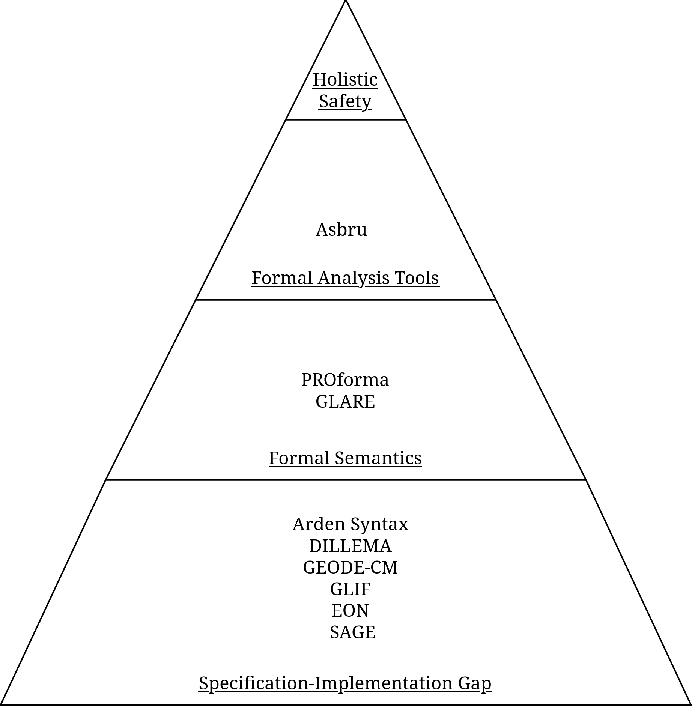
\includegraphics[width=0.5\textwidth]{pyramid}
  \caption{Existing \DSLs{} for Computer Interpretable Guidelines}\label{fig:existing-work-pyramid}
\end{figure}

Over the years, significant progress has been made towards
addressing these challenges. In \autoref{chapter:related-work},
we discussed how existing approaches have attempted to
address said challenges, and their limitations. Specifically,
in \autoref{sec:related-work-discussion}, we outlined major
themes that these approaches adopt to tackle these challenges.
This is further illustrated by the pyramid diagram in \autoref{fig:existing-work-pyramid}, where aforementioned themes are
underlined in the pyramid's various rungs.
As is typical, approaches that appear in higher rungs also
have characteristics of ones below them. For example, while guidelines expressed in
the Arden Syntax eliminate the specification-implementation gap by being
both \HCP{}-comprehensible and interpretable, they cannot be formally analyzed
due to lack of analysis tools in the ecosystem. Asbru-based guidelines
on the other hand not only eliminate the specification-implementation gap, but can also be
formally analyzed using support for KIV-based verification in the Asbru
ecosystem (see \autoref{sec:kiv-verification}).

As is evident in \autoref{fig:existing-work-pyramid}, no
existing approach covers the \say{holistic safety} rung of the pyramid.
Recall from \autoref{sec:related-work-discussion} that we say an
approach tackles \say{holistic safety} if,
besides support for analyzing guidelines,
analysis and execution tools also have correctness guarantees.
In this work, we argue that such guarantees are necessary for
trustworthy \CDSSs{}. We attempt to address \say{holistic safety}
systematically by developing a \emph{semantics-first approach} for
building clinical decision support systems. In this context, by semantics-first
we mean that:
\begin{itemize}
  \item The semantics of the programming language for defining said knowledge is
    formally defined, from which execution and analysis tools are derived in a
    correct by construction manner, leading to holistic safety.
  \item The semantics of medical knowledge are expressed accurately.
\end{itemize}
At the core of our approach is a novel domain-specific language for expressing
medical knowledge called $\MediK{}$ (pronounced Medi-Kay). By being comprehensible to domain experts
in medicine, $\MediK{}$-based computer interpretable guidelines can serve
both as a guideline's non-executable \HCP{}-comprehensible description, i.e.,
the specification, and its encoding in a computable medium, i.e., the
implementation, thereby eliminating any specification-implementation gap.

The remainder of this chapter is structured as follows:
\autoref{sec:semantics-first} briefly describes the semantics-first philosophy.
Next, \autoref{sec:k-framework} describes $\K$ -- the language semantic
framework that $\MediK{}$'s are expressed in. Finally,
\autoref{sec:semantics-first-pitfalls} describes potential pitfalls
of following the semantics-first philosophy.

\section{Semantics-First Approach}\label{sec:semantics-first}

The semantics-first approach prescribes a systematic way of
developing programming languages. Instead of implementing
tools for a language, such as interpreters, compilers and
model checkers in ad-hoc manner, the approach states that the
first step in developing said tools must be to formally define
the language's semantics. As show in \autoref{fig:semantics-first},
once defined, all tools for the language
can then be automatically derived from the semantics. Moreover, since
the tools utilize the semantics, they are, by definition,
correct-by-construction.

While following the semantics-first philosophy might seem like an obvious choice
in language design, its adoption in practice is far from ideal.
Conventional practice in the programming language and formal
methods community is still to develop analysis and execution tools for each
programming language from scratch \cite{ChenSETSS19}, as illustrated
in \autoref{fig:conventional-pl-development} from
\cite{ChenSETSS19}. But, this approach has several
disadvantages:
\begin{itemize}
  \item Implementing tools that perform the same function for
    different languages incurs unnecessary development and maintenance cost.
    As shown in \autoref{fig:conventional-pl-development}, if there are
    $l$ languages, where each has $t$ tools, then a total of $l \times t$
    tools have to be developed and maintained over time.
  \item Tools are often based on informal descriptions of language semantics,
    leaving developers to extrapolate finer details of the language's semantics,
    leading to inconsistencies.
    For instance, in \cite{ParkPLDI15}, it was found
    that ECMAScript 5.1-compliant JavaScript engines
    in mainstream web browsers behaved differently from each other
    for certain complex JavaScript programs.
  \item As newer versions of a language are introduced, each
    tool for the language has to be updated to ensure support for the latest
    version. This again results in duplicated work.
\end{itemize}
\begin{figure}[t!]
  \centering
  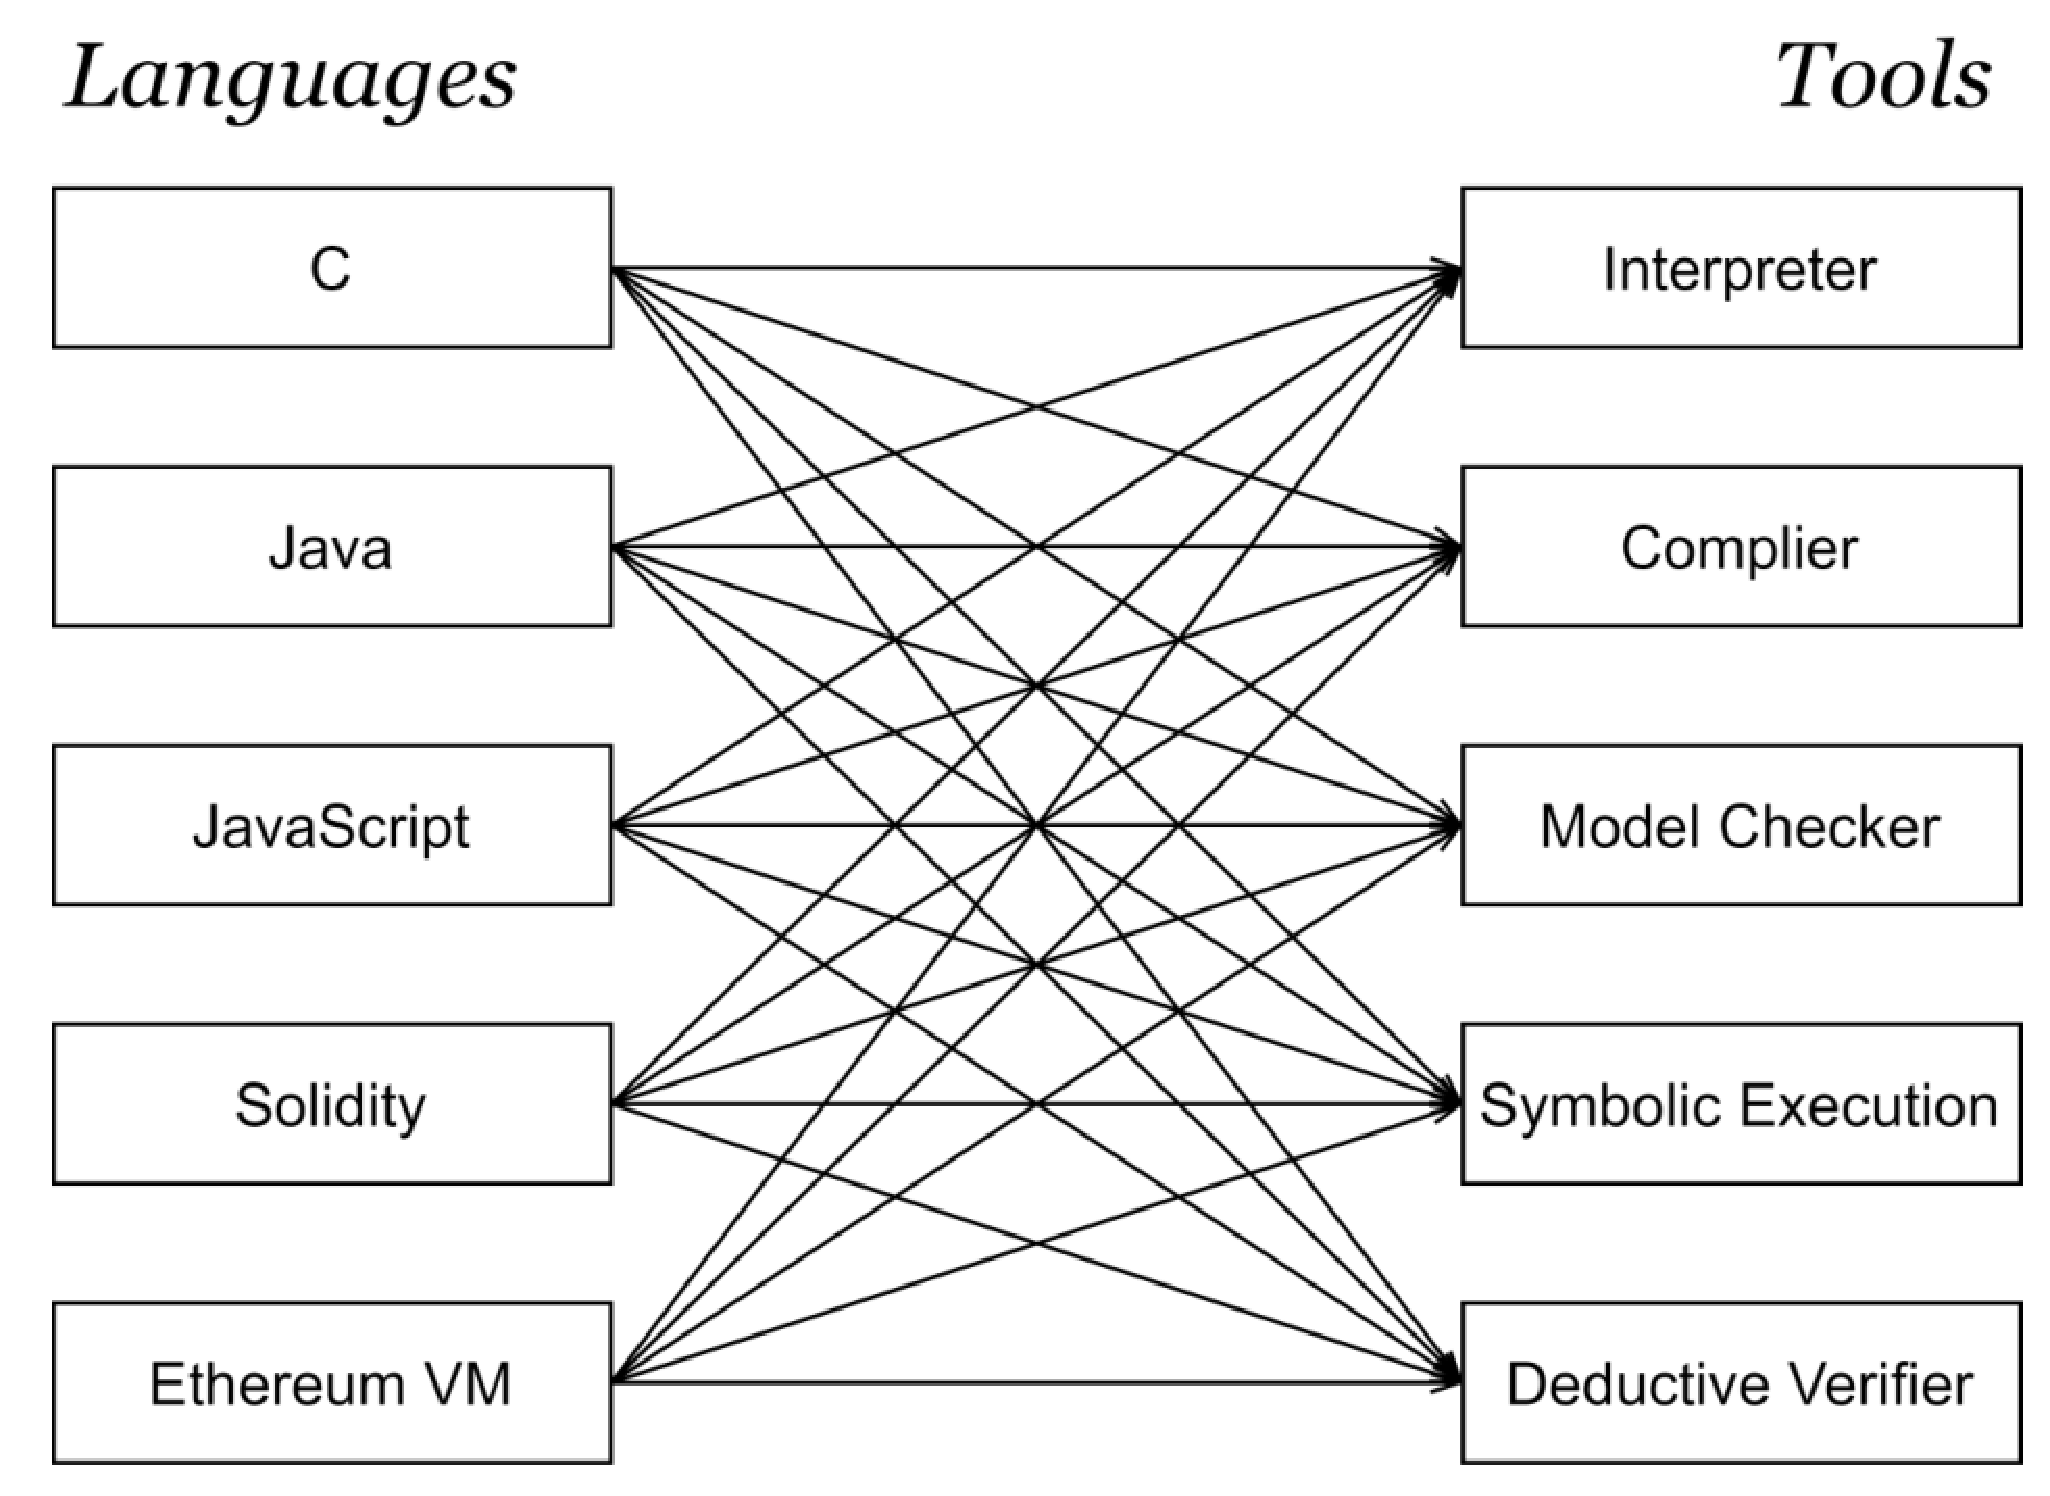
\includegraphics[width=0.6\textwidth]{conventional-pl-development}
  \caption{State-of-Art in Programming Language Design}\label{fig:conventional-pl-development}
\end{figure}

\subsection{Why build \CDSSs{} using Semantics-First?}

In section \ref{sec:semantics-first}, we described benefits
of using the semantics-first approach for developing regular programming
language. But, these differences become starker when semantics-first
is compared against the conventional approach shown in \autoref{fig:conventional-pl-development} in context of domain-specific language for
expressing medical guidelines. Specifically, as such a language will be utilized
in safety-critical settings, it is vital that the language:
\begin{itemize}
  \item Has an \emph{unambiguous}, \emph{formal}
    semantics that can serve as a reference for developing tool support for it.
    This is necessary to ensure that
    tools are free of behavioral inconsistencies due to ambiguities in the
    semantics.
  \item Is supported by a rich formal analysis tools that can
    be used to analyze programs.
    Implementing such tools from scratch would require significant effort.
  \item Can evolve quick to incorporate
    \begin{enumerate*}[label=(\roman*)]
      \item lessons from expressing medical guidelines in it, and,
      \item \HCP{} feedback, specifically regarding comprehensibility.
    \end{enumerate*}
    This can be challenging when using the approach shown in \autoref{fig:conventional-pl-development}, as
    every change to the language's semantics would require corresponding
    changes to all relevant tools, and additional effort to maintain
    different versions, making the development process extremely tedious.
\end{itemize}

\section{The $\K{}$ Framework}\label{sec:k-framework}

In this section, we introduce $\K{}$: a rewrite-based executable semantics
in which programming languages can be defined through configurations and rules
\cite{KframeworkUrl}. Once the semantics of a programming language has been
defined, $\K{}$ automatically generates all tools depicted in \autoref{fig:semantics-first}, such as an interpreter, compiler,
model-checker and deductive verifier for the language. $\K{}$ has been successfully
utilized to formalize semantics of large real-world languages, such as
C \cite{HathhornPLDI15}, Java \cite{BogdanasPOPL15} and
Javascript \cite{ParkPLDI15}, and analyze non-trivial programs
\cite{StefanescuOOPSLA16,ParkFSE18}.

The remainder of this section introduces relevant features of
$\K{}$ by describing the $\K{}$ semantics of an example language called
Imp. This introduction to $\K{}$ provides necessary background
for upcoming chapters that discuss the $\MediK{}$ \DSL{} through the
use of $\K{}$ notation and concepts.

\subsection{Defining Languages in $\K$}\label{sec:semantics-in-k}

A typical $\K$ definition of a language consists of the following components:
\begin{itemize}
  \item Syntax: Defined in \BNF{}-like notation, and utilized by $\K$
    to generate a parser for the language.
  \item Configuration: Organizes the program execution state
    into units called \emph{cells} that may be nested.
  \item Rules: Operate over configuration segments and define program
    evolution via rewrites.
\end{itemize}
We now discuss aforementioned components in the context of the Imp
language. Imp is a simple imperative programming language
inspired by C and Java that supports arithmetic and boolean expressions and
statements such as variable declaration and assignment, branching (\inlineimp{if})
and looping (\inlineimp{while}).

\autoref{lst:imp-syntax} and \autoref{lst:imp-semantics},
define syntax and semantics of Imp respectively.
$\K{}$ code must be place inside an organizational unit called a
\inlinek{module} that has a name, and can import other \inlinek{module}(s).
For example, \inlinek{module IMP-SYNTAX ... endmodule}
between \autoref{lstline:imp-module-start} and
\autoref{lstline:imp-module-end} of \autoref{lst:imp-syntax} defines
a $\K{}$ \inlinek{module} named \inlinek{IMP-SYNTAX} containing Imp's
grammar. $\K{}$ provides builtin support for domains such as natural
numbers, integers, booleans and program identifiers
under a \inlinek{module} named \inlinek{DOMAINS}.
\autoref{lstline:imp-syntax-import} \inlinek{imports}
the syntax definition of $\K{}$'s \inlinek{DOMAINS} module
to enable parsing integers and booleans in Imp programs.

\begin{lstlisting}[float=ht,
  frame=single,
  style=ksty,
  language=k,
  numbers=left,
  numbersep=5pt,
  caption={Imp Syntax in $\K$},
  label={lst:imp-syntax}
]
module IMP-SYNTAX                                               @\label{lstline:imp-module-start}@
  imports DOMAINS-SYNTAX                                        @\label{lstline:imp-syntax-import}@
  syntax AExp  ::= Int | Id                                     @\label{lstline:imp-aexp-start}@
                 | "-" Int
                 | AExp "/" AExp              [left, strict]    @\label{lstline:imp-aexp-div}@
                 | "(" AExp ")"               [bracket]
                 > AExp "+" AExp              [left, strict]    @\label{lstline:imp-aexp-end}@
  syntax BExp  ::= Bool
                 | AExp "<=" AExp             [seqstrict]
                 | "!" BExp                   [strict]
                 | "(" BExp ")"               [bracket]
                 > BExp "&&" BExp             [left, strict(1)] @\label{lstline:imp-bexp-and}@
  syntax Block ::= "{" "}"
                 | "{" Stmt "}"
  syntax Stmt  ::= Block                                        @\label{lstline:imp-stmt-block}@
                 | Id "=" AExp ";"            [strict(2)]       @\label{lstline:imp-stmt-assgn}@
                 | "if" "(" BExp ")"
                   Block "else" Block         [strict(1)]
                 | "while" "(" BExp ")" Block                   @\label{lstline:imp-stmt-while}@
                 > Stmt Stmt                  [left]            @\label{lstline:imp-stmt-comp}@
  syntax Pgm ::= "int" Ids ";" Stmt                             @\label{lstline:imp-pgm}@
  syntax Ids ::= List{Id,","}                                   @\label{lstline:imp-ids}@
endmodule                                                       @\label{lstline:imp-module-end}@
\end{lstlisting}

\emph{Syntax} in $\K{}$ is defined using BNF-like notation; terminals are enclosed
in quotes, and non-terminals begin with an uppercase. For example,
consider the declaration of Imp arithmetic expressions between
\autoref{lstline:imp-aexp-start} and \autoref{lstline:imp-aexp-end}. On
\autoref{lstline:imp-aexp-start} $\K$'s builtin support
for integers (\inlinek{Int}) and program identifiers
(\inlinek{Id}) is used to support arithmetic expressions over program variables.
Beyond simply defining the syntax, $\K{}$ also allows assigning semantics to
constructs through the use of \emph{attributes} specified as a comma-separated list
inside square brackets (\inlinek{[..]}) placed immediately after the \BNF{} production.
For example, On \autoref{lstline:imp-aexp-div} and \autoref{lstline:imp-aexp-end},
the attribute \inlinek{left} is used to declare the
corresponding operator as left associative. The \inlinek{strict} attribute is used
to assign \emph{evaluation strategies}. Note its use
on \autoref{lstline:imp-aexp-div} and \autoref{lstline:imp-aexp-end}, signifying
that both operand sub-expressions must be completely evaluated before the
before the corresponding operator (\inlinek{/}, \inlinek{+}) is evaluated.
Note that the order in which the arguments are evaluated is non-deterministic,
and, all operands will be evaluated before the operator is evaluated.
To enforce a particular order, or, to choose a subset of the operands, a
list of operand positions specifying the desired order can be supplied to
\inlinek{strict}. For example, \inlinek{strict(2, 1)} would make $\K$
evaluate the second argument before the first. This is particularly
useful for defining constructs like short-curcuit (\inlineimp{&&}) boolean
expression on \autoref{lstline:imp-bexp-and}, where \inlinek{strict(1)}
ensures that the left operand is evaluated first, allowing the right to only
be evaluated if the left evaluates to \inlinek{true}.
Similarly, for an assignment statement on \autoref{lstline:imp-stmt-assgn}
the \inlinek{strict(2)} indicates that the second argument, i.e., the
expression to the right of the \inlineimp{=} sign must be evaluated before
the identifier on the left of the \inlineimp{=} is updated.

$\K{}$ also allows operator precedence to be specified as a part of the
syntax definition. On \autoref{lstline:imp-aexp-end},
the \inlinek{>} signifies that all preceding productions have higher precedence,
i.e., bind tighter, than the production for addition (\inlinek{+}).
Similarly, \autoref{lstline:imp-stmt-comp} defines statement composition.
Thus, preceding \inlinek{Stmt} productions
(\autoref{lstline:imp-stmt-block}-\autoref{lstline:imp-stmt-while}), that define
blocks (\inlinek{\{..\}}) and standalone statements such as variable assignment and
while loop have higher precedence, indicated by \inlinek{>} on \autoref{lstline:imp-stmt-comp}.

On \autoref{lstline:imp-pgm}, an Imp program is defined to start with a list of program variable
declarations (\inlinek{"int" Ids ";"}) followed by other statements. Note the
definition of a list of identifier (\inlinek{Ids}) on \autoref{lstline:imp-ids}. In $\K{}$,
\inlinek{List\{...\}} is used to define syntactic-lists, where the first
argument is the production of list elements, and the second the list de-limiter.
Thus, \inlinek{List\{Id, ","\}} defines a comma-separated list of program identifiers.

Once the \emph{syntax} has been defined, $\K$ can utilize it to generate a
parser, which can be used to generate abstract
syntax trees (\ASTs{}) for programs. The program's \AST{} forms a part of the larger
program state, over which semantics are defined through rules.
The $\K$ semantics of any language has two components:
\begin{itemize}
  \item A \emph{Configuration} that organizes the state
    into units called \emph{cells}, that may be nested.
  \item \emph{Rules} that operate over \emph{configuration}-segments
    to desribe evolution of state during execution.
\end{itemize}
For Imp, \autoref{lst:imp-semantics} has aforementioned
components inside \inlinek{module IMP}.
Note that the syntax and semantics exist in separate modules,
where the semantics module \inlinek{imports}
the syntax module. This is by convention, and
has the following advantages:
\begin{enumerate}[label=\alph*)]
  \item Rules can operate directly over the language's syntax,
    making them easier to specify and comprehend.
  \item With the syntax and semantics residing in separate modules,
    $\K$ can be instructed to use only the syntax module for parsing programs.
    This allows users to define additional syntactic constructs in the semantics module
    for use in rules. If a combined syntax and semantics module is used instead,
    any constructs defined solely for use in rules
    would unintentionally become part of the language's syntax,
    and be accepted by the parser.
\end{enumerate}

\begin{lstlisting}[float=t,
  frame=single,
  style=ksty,
  language=k,
  numbers=left,
  numbersep=5pt,
  caption={$\K$ Semantics of Imp},
  label={lst:imp-semantics}
]
module IMP
  imports IMP-SYNTAX
  imports DOMAINS
  syntax KResult ::= Int | Bool             @\label{lstline:imp-kresult}@

  configuration <T>                         @\label{lstline:imp-config-start}@
                  <k> $PGM:Pgm </k>         @\label{lstline:imp-pgm-var}@
                  <state> .Map </state>     @\label{lstline:imp-pgm-state}@
                </T>                        @\label{lstline:imp-config-end}@

// AExp
  rule <k> X:Id => I ...</k> <state>... X |-> I ...</state> @\label{lstline:imp-assgn-rule}@
  rule I1 / I2 => I1 /Int I2  requires I2 =/=Int 0
  rule I1 + I2 => I1 +Int I2                @\label{lstline:imp-add-rule}@
  rule - I1 => 0 -Int I1
// BExp
  rule I1 <= I2 => I1 <=Int I2
  rule ! T => notBool T
  rule true && B => B
  rule false && _ => false
// Block
  rule {} => .   [structural]
  rule {S} => S  [structural]
// Stmt
  rule <k> X = I:Int; => . ...</k> <state>... X |-> (_ => I) ...</state>
  rule S1:Stmt S2:Stmt => S1 ~> S2  [structural] @\label{lstline:imp-stmt-decomp}@
  rule if (true)  S else _ => S  @\label{lstline:imp-if-true-rule}@
  rule if (false) _ else S => S  @\label{lstline:imp-if-false-rule}@
  rule while (B) S => if (B) {S while (B) S} else {}  [structural]
// Pgm
  rule <k> int (X,Xs => Xs);_ </k> <state> Rho:Map (.Map => X|->0) </state> @\label{lstline:imp-vardec-rule}@
    requires notBool (X in keys(Rho))  @\label{lstline:imp-vardec-requires}@
  rule int .Ids; S => S  [structural]  @\label{lstline:imp-emptydec-rule}@

endmodule
\end{lstlisting}

\subsubsection{Configurations}\label{sec:k-configuration}

The configuration is defined using the keyword \inlinek{configuration},
followed by an unordered list of \emph{cells},
which may be nested and are specified using an XML-like notation.
For instance, \inlinek{<foo> <bar> ... </bar> </foo>}
corresponds to $\K$ \emph{cells} named
\inlinek{foo} and \inlinek{bar} respectively, where \inlinek{bar}
is nested under \inlinek{foo}.
Imp's configuration is defined
between \autoref{lstline:imp-config-start} and \autoref{lstline:imp-config-end},
and consists of a top-level cell \inlinek{<T>} containing cells
\inlinek{<k>} and \inlinek{<state>} on \autoref{lstline:imp-pgm-var} and
\autoref{lstline:imp-config-end} respectively. In $\K{}$,
the \inlinek{<k>} cell typically contains the \AST{} of the executing
program, indicated by its contents \inlinek{$PGM:Pgm}.
During execution, $\K{}$ will attempt to parse the program being executed
using the production \inlinek{Pgm} defined on \autoref{lstline:imp-pgm} of
\autoref{lst:imp-syntax}. If parsing is successful, $\K{}$ will replace
\inlinek{$PGM} with the parsed \AST{}. The \inlinek{<state>} cell,
as the name suggests, will hold a map of
program identifiers and values they acquire during execution.
Said map is initially empty, denoted by \inlinek{.Map}.
The dot (\inlinek{.}) in $\K{}$ denotes \emph{nothing} or \emph{empty}.
Thus, \inlinek{.Map} denotes an empty map.

\subsubsection{Rules}\label{sec:k-rules}
$\K$ \emph{rules} operate over configuration segments and define evolution of
program state. When specifying a rule $\K{}$, only relevant parts of the
configuration need to be mentioned---$\K{}$ completes the rest of the
configuration through a mechanism called \emph{configuration abstraction}.
This allows rules to be concise,
enhancing readability and making them easier to write. For example,
consider the rule for addition on \autoref{lstline:imp-add-rule}.
Simply put, the rule specifies that if the term at the top of the \inlinek{<k>}
cell is an addition expression, then it should be \emph{rewritten} to
addition in the integer domain \inlinek{+Int}. But, even though the
rule is intended to simplify the top of the \inlinek{<k>} cell,
no cells are explicitly mentioned. This is because:
\begin{itemize}
  \item If no cell is mentioned, $\K$ assumes that rule applies at the top of
    the $\K{}$ cell.
  \item All other parts of the configuration are assumed to remain unchanged.
\end{itemize}

Now we describe rules in greater depth.
A rule begins with the keyword \inlinek{rule}
and is a statement of the form $\varphi \To \psi$, where
$\varphi$, $\psi$ are \emph{patterns} over configuration terms and $\K$ variables.
We say $\varphi$ is the LHS and $\psi$ is the RHS of the rule.
We define a \emph{substitution} $\theta$ to be a map from $\K$-variables to terms.
Given pattern $\varphi$ and \emph{substitution} $\theta$, we say
$\varphi\theta$ is the pattern obtained by replacing every variable $v$ in
$\varphi$ with $\theta(v)$. We say pattern $\varphi$ matches
term $\tau$ iff there exists a substitution $\theta$ s.t. $\tau = \varphi\theta$.
During execution, if the current configuration term
$\tau$ \emph{matches} the LHS $\varphi$ of rule $\varphi \To \psi$
with substitution $\theta$, then $C$ is rewritten to $\psi\theta$.
For example, the addition rule on \autoref{lstline:imp-add-rule}.
$\K$-variables always begin with an uppercase, and may be suffixed with
\inlinek{:S}, where \inlinek{S} is the variable's sort. In the case
of the addition rule, $\K$ can \emph{infer} that the sort of
\inlinek{I1} and \inlinek{I2} is \inlinek{Int}, as operands of the
buitin operator \inlinek{+Int} can only be integers (\inlinek{+Int}
is addition in the domain of integers). Thus, the \LHS{} \inlinek{I1 + I2}
\emph{match} term \inlinek{2 + 3} (of sort \inlinek{AExp})
with substitution
\inlinekmath{$\theta = $(I1\ $\mapsto$ 2, I2\ $\mapsto$\ 3)} and rewrite it \inlinek{2 +Int 3}, i.e. \inlinek{5}, as
\inlinek{+Int} is $\K$-builtin for integer addition.

We now discuss execution of an entire program to introduce $K{}$ nuances
relevant to later chapter. Imp's grammar dictates that an
Imp program (denoted by production \inlinek{Pgm} on
\autoref{lstline:imp-pgm} of \autoref{lst:imp-syntax})
must declare all variables at the start of execution. Consider
the simple program \inlinemedik{int x; x = 2 + 3;}.
At the start of execution, \K{} replaces the \inlinek{$PGM}
in the configuration declaration with the program's \AST{}.
Thus, we get the following initial configuration:
\begin{lstlisting}[language=k,style=ksty,backgroundcolor=\color{white}]
<T>
  <k> int x, .Ids; x = 2 + 3; </k>
  <state> .Map </state>
</T>
\end{lstlisting}
where \inlinek{.Ids} is the identity element for the user-defined
list of program identifiers, and \inlinek{.Map} is the map identity
from the initial configuration declaration on \autoref{lstline:imp-pgm-state}
Now the rule for variable declaration on \autoref{lstline:imp-vardec-rule}
can match with substition \inlinekmath{(X $\ \mapsto\ $ x, Xs\ $ \mapsto\ $ .Ids,
Rho $\ \mapsto\ $.Map)}
to rewrite the configuration to:
\begin{lstlisting}[language=k,style=ksty,backgroundcolor=\color{white}]
<T>
  <k> int .Ids; x = 2 + 3; </k>
  <state> x |-> 0 </state>
</T>
\end{lstlisting}
Note the following conveniences that \K{} offers to make writing rules easier:
\begin{enumerate}[label=\roman*)]
  \item The use of parenthesis limi scope of the rewrite to the
    list of program identifiers. Localized rewriting reduces redundancy
    as only relevant parts of a term have to be mentioned on the \RHS{} of the
    rule.
  \item The underscore \inlinek{_} following \inlinek{int (X, Xs => Xs);}
    on \autoref{lstline:imp-vardec-rule}
    is an \emph{anonymous} variable that matches the remainder to the program.
    Since it's not anywhere on the \RHS{}, there is no need to provide an
    explicit variable name.
\end{enumerate}
Also that the rule has a side condition, expressed through the keyword \inlinek{requires}
on \autoref{lstline:imp-vardec-requires}. This forces the rule to only apply if
the program identifier has not already been declared. For instance,
a program that starts with \inlineimp{int x, x;} will not execute to completion.
Next, the rule on \autoref{lstline:imp-emptydec-rule} will eliminate
\inlinek{int .Ids;}, leaving the following configuration after the rewrite:
\begin{lstlisting}[language=k,style=ksty,backgroundcolor=\color{white}]
<T>
  <k> x = 2 + 3; </k>
  <state> x |-> 0 </state>
</T>
\end{lstlisting}
Also note that the rule does not explicitly mention the cell on which
it is intended to operate. In $\K$, a rule that doesn't
mention any cells is implicitly assumed to apply on top of the
\inlinek{<k>} cell. As the \inlinek{<k>} cell typically
contains the program being executed, not having to explicitly
mention the cell allows the rule to only show how constructs in the language
affect execution. For instance, the rules on \autoref{lstline:imp-if-true-rule}
and \autoref{lstline:imp-if-false-rule} depict that for an
\inlineimp{if(condition) \{...\}} statement,
if the \inlineimp{condition} is true, the \inlineimp{if} block is taken,
else whatever comes after is taken.

Next, consider the assignment rule on \autoref{lstline:imp-assgn-rule} of
\autoref{lst:imp-semantics}. The rule uses two variables: \inlinek{X} and \inlinek{I}
with sorts \inlinek{Id} and \inlinek{Int} respectively. Since the \inlinek{<k>}
cell in our running example has \inlinek{x = 2 + 3;}, we expect the assignment
rule to apply at some point and update the \inlinek{<state>} accordingly.
But, the rule cannot apply as the \RHS{} of the assignment, i.e., the expression
\inlinek{2 + 3}, is not of sort \inlinek{Int}, which needs to be evaluated
first. This in \K{} is enabled by evaluation strategies.
Recall that the attribute assignment statement has the attribute
\inlinek{strict(2)} (\autoref{lstline:imp-stmt-assgn} of
\autoref{lst:imp-syntax}), denoting that the second argument of the
construct must be evaluated first. Thus,
$\K$ will \emph{heat}, or pull-out the second
argument for evaluation. This results in the configuration:
\begin{lstlisting}[language=k,style=ksty,backgroundcolor=\color{white}]
<T>
  <k> 2 + 3 ~> x = []; </k>
  <state> x |-> 0 </state>
</T>
\end{lstlisting}
In $\K{}$, \lstinline[style=inlineksty]{~>} means \emph{followed-by}, i.e.,
the evaluation of \inlinek{2 + 3} must occur \emph{before} the evaluation
of \inlinek{x = [];}. \inlinek{[]} denotes a \emph{hole} left in place of
the argument that was \emph{heated}.
\inlinek{<k> 2 + 3 ~> x = []; </k>}
is re-written to \inlinek{<k> 5 ~> x = []; </k>}
by an application of the arithmetic addition rule on
\autoref{lstline:imp-add-rule}. On
\autoref{lstline:imp-kresult},
we specify any term of sort \inlinek{Int} to be a \inlinek{KResult}.
This signifies that the term can no longer be evaluated, and can be \emph{cooled}
or plugged-back into its corresponding hole, resulting in the configuration:
\begin{lstlisting}[language=k,style=ksty,backgroundcolor=\color{white}]
<T>
  <k> x = 5; </k>
  <state> x |-> 0 </state>
</T>
\end{lstlisting}
Now the LHS of the assignment rule can \emph{match} with substitution
\inlinekmath{$\theta$\ =\ (X\ $\mapsto$\ x, I\ $\mapsto$\ 5)}
 resulting in the final configuration:
\begin{lstlisting}[language=k,style=ksty,backgroundcolor=\color{white}]
<T>
  <k> . </k>
  <state> x |-> 5 </state>
</T>
\end{lstlisting}

Note the difference between program identifiers and $\K$ variables. While
program variables are simply terms belonging to sort \inlinek{Id},
$\K$ variables have logical meaning. If multiple rules can match
the configuration term, then one rule is non-deterministically chosen.
Execution is a sequence of rule applications that continues until no
rule can match the configuration. Since in the running example the
$\K{}$ the \inlinek{<k>} cell becomes empty after all statement are evaluated,
indicating successful completion.

\section{Pitfalls of the Semantics-First Approach}\label{sec:semantics-first-pitfalls}



% per Graduate College preference, place the \appendix and the appendices content before the
% bibliography (here) only if the appendices contain references.

\backmatter

\printbibliography[heading=bibintoc,title={References}]

% the below lines are only needed if bibliography precedes appendices
% uses https://tex.stackexchange.com/a/440212 to continue page numbering
\clearpage
\setcounter{counterforappendices}{\value{page}}
\mainmatter
\setcounter{page}{\value{counterforappendices}}

\appendix

\chapter{An appendix}


% \input{Appendix.tex}

\end{document}
